
\subsection{Phân tích phương sai hai nhân tố (Two-factor ANOVA)}
\subsubsection{Mục đích}
Trong phần nghiên cứu này, chúng tôi sẽ sử dụng ANOVA 2 yếu tố không lặp để phân tích xem liệu \textbf{Được giao hàng nhanh (is\_expedited\_delivery)} và \textbf{Mùa (season)} có ảnh hưởng đến \textbf{Phí giao hàng (delivery\_charges)} hay không?

Giả thiết thống kê được thực hiện với mức ý nghĩa $\alpha = 0.05$.


\begin{itemize}
    
    \item Kiểm định yếu tố A (is\_expedited\_delivery)
    \begin{itemize}
        \item Đánh giá xem biến nhân tố A có ảnh hưởng đến biến phụ thuộc hay không?
        
        \[
            H_{0A}: \tau_{1} = \tau_{2} = \tau_{3} = \dots = \tau_{a} = 0
            \]
            \[
            H_{1A}: \tau_{i} \neq  0 \text{ với ít nhất một i }
            \]
    \end{itemize}
    Các mùa (season) có ảnh hưởng rất mạnh đến phí giao hàng (delivery\_charges).
    
    \item Kiểm định yếu tố B (season)
    \begin{itemize}
        \item Đánh giá xem biến nhân tố B có ảnh hưởng đến biến phụ thuộc hay không?
        
        \[
            H_{0B}: \beta_{1} = \beta_{2} = \beta_{3} = \dots = \beta_{b} = 0
            \]
            \[
            H_{1B}: \beta_{j} \neq  0 \text{ với ít nhất một j }
            \]
    \end{itemize}
    Việc khách hàng yêu cầu giao hàng nhanh (is\_expedited\_delivery) có ảnh hưởng rất mạnh đến phí giao hàng (delivery\_charges).
    \item Đối với tương tác giữa A và B  
    \begin{itemize}
        \item Đánh giá xem các biến nhân tố A và B có tương tác với nhau hay không?
        
        \[
            H_{0AB}: \tau\beta_{11} = \tau\beta_{12}  = \dots = \tau\beta_{AB} = 0 
            \]
            \[
            H_{1AB}: \tau\beta_{ij} \neq  0 \text{ với ít nhất một cặp (i,j) }
            \]
    \end{itemize}
\end{itemize}
\subsubsection{Kiểm tra điều kiện cho dữ liệu}
Trước khi tiến hành phân tích ANOVA 2 chiều, ta cần kiểm tra các điều kiện cần thiết cho dữ liệu:


 Đầu tiên ta kiểm tra xem dữ liệu của \textbf{Biến phụ thuộc:} \textbf{delivery\_charges} ở mỗi nhóm do tổ hợp các mức của hai nhân tố tạo ra có tuân theo phân phối chuẩn không.
 \begin{figure}[!htbp]
    \centering
    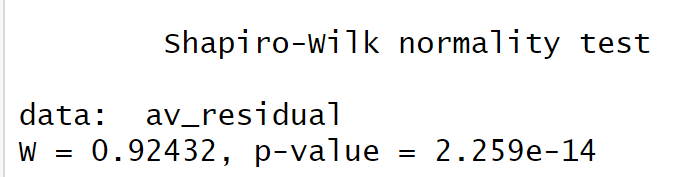
\includegraphics[width=0.7\linewidth]{graphics/5.4.1 (2).png}
    \caption{Kết quả kiểm tra phân phối chuẩn}
\end{figure}

Có thể thấy p\_value < 0. 05 dữ liệu không tuân theo phân phối chuẩn.
Tuy dữ liệu không tuân theo quy luật phân phối chuẩn nhưng mẫu đủ lớn, ta vẫn có thể sử dụng mô hình anova mà không cần lo ngại quá nhiều về vấn đề phân phối chuẩn của dữ liệu. Điều này dựa trên lý thuyết \textbf{Lý thuyết Giới hạn Trung tâm (Central Limit Theorem - CLT)}. 


   Tiếp theo, ta kiểm tra xem các nhóm được phân tích ở trên có phương sai đồng nhất hay ko 

   \begin{figure}[!htbp]
    \centering
    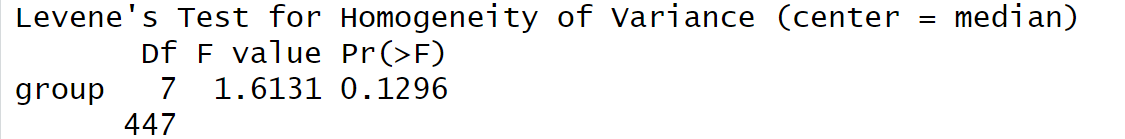
\includegraphics[width=0.7\linewidth]{graphics/5.4.2.png}
    \caption{Kết quả kiểm tra phương sai đồng nhất}
\end{figure}

Có thể thấy giá trị p > 0.05 nên các nhóm có phương sai đồng nhất . 
Sau khi đã thỏa mãn các điểu kiện kiểm tra dữ liệu ta tiến hành phân tích ANOVA 2 chiều.

\subsubsection{Tiến hành phân tích}


        Dựa vào bảng dữ liệu ta có thể thấy sự tương tác giữa 2 nhân tố is\_expedited\_delivery và season

        \begin{figure}[!htbp]
            \centering
            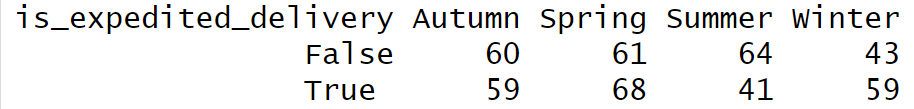
\includegraphics[width=1\linewidth]{graphics/5.4.3.png}
            \caption{bảng dữ liệu}
        \end{figure}
        Kết quả nhận được: 

        \begin{figure}[!htbp]
            \centering
            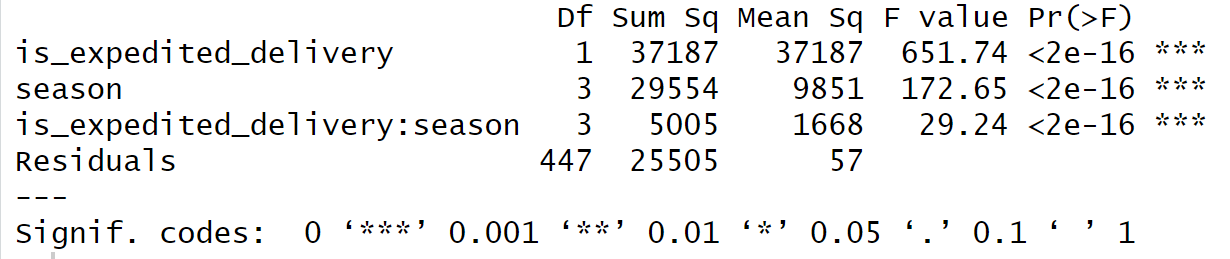
\includegraphics[width=1\linewidth]{graphics/5.4.4.png}
            \caption{Phân tích anova 2 yếu tố}
        \end{figure}

        Chúng tôi tiến hành phân tích ANOVA 2 chiều trong phần phần mềm r. 
        Kết quả và nhận xét: 
        Kết quả phân tích ANOVA hai yếu tố được trình bày trong hình 5.7. Kết quả cho thấy rằng cả ba yếu tố \textbf{season}, \textbf{is\_expedited\_delivery}, và sự tương tác giữa chúng đều có ảnh hưởng đáng kể đến \textbf{delivery\_charges} với mức ý nghĩa $\alpha = 0.05$. Dưới đây là các nhận xét chi tiết:

        \begin{itemize}
    \item \textbf{Tương tác giữa season và is\_expedited\_delivery}:
    \begin{itemize}
        \item Với \textbf{Df = 3}, có 3 mức độ tương tác giữa hai yếu tố \textbf{season} và \textbf{is\_expedited\_delivery}.
        \item Giá trị \textbf{F = 29.24} và \textbf{Pr(>F) = 2e-16***} cho thấy rằng có sự tương tác có ý nghĩa thống kê giữa hai yếu tố này và ảnh hưởng đến \textbf{delivery\_charges}. Do đó, ta bác bỏ giả thuyết không \(H_0\) cho sự tương tác này.
    \end{itemize}

    \end{itemize}

 Từ những kết quả trên, chúng tôi kết luận rằng cả yếu tố \textbf{season}, \textbf{is\_expedited\_delivery}, và sự tương tác giữa chúng đều có ảnh hưởng quan trọng và có ý nghĩa thống kê đối với \textbf{delivery\_charges}. Điều này cho thấy rằng các yếu tố này cần được cân nhắc kỹ lưỡng khi định giá sản phẩm.
               
        
\subsubsection{Kết luận}
Phân tích ANOVA 2 chiều cho thấy \textbf{season}, \textbf{is\_expedited\_delivery}, và sự tương tác giữa chúng đều có ảnh hưởng đáng kể đến \textbf{delivery\_charges}. Mặc dù có một số hạn chế về phân phối chuẩn , kết quả này vẫn cung cấp cơ sở tin cậy để đánh giá và điều chỉnh chiến lược giá sản phẩm.